There is an ongoing effort at the 3GPP on giving \gls{wrtc} clients access to \gls{ims} with 3GPP TR 23.701\cite{3gpp-wrtc-access-ims} as the current proposed architecture. \gls{ims} is basically an architectural framework for delivering IP multimedia services. It was originally designed for evolving mobile networks beyond \gls{gsm}. Later it has evolved to include Wireless LAN and fixed lines, it's intended to aid the access of multimedia and voice applications across different networks. This study is relevant because most telecom companies already have IMS or a similar architecture in place for doing real-time communication. You have to read the report\cite{3gpp-wrtc-access-ims} to understand all the different components. The following diagram shows the proposed architecture:

\begin{figure}[here]
\centerline{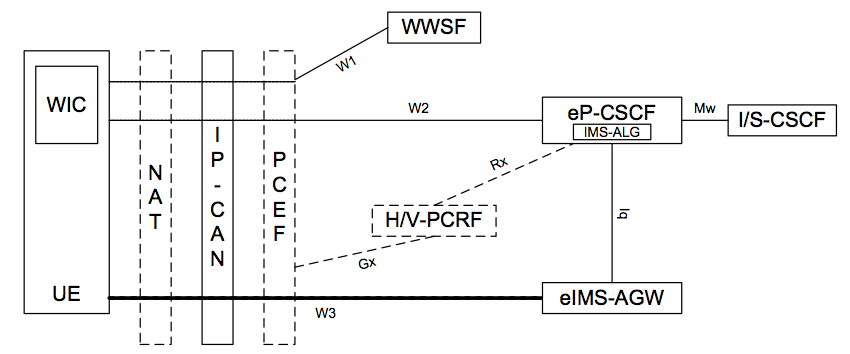
\includegraphics[scale=0.5]{3gpp-wrtc-ims-architecture.png}}
\caption{WebRTC IMS architecture by 3GPP TR 23.701 as work in progress.}
\label{fig:wrtc-ims-architecture}
\end{figure}

\subsection{Doubango Telecom}
Doubango Telecom has created a Smart SIP and Media Gateway to connect WebRTC endpoints\footnote{http://webrtc2sip.org/}. It's called webrtc2sip and it uses RTCWeb and SIP technologies. It allows your browser to make and receive calls to and from any SIP endpoint. The gateway contains four modules: a SIP Proxy, a RTCWeb Breaker, a Media Coder, and a Click-to-Call service. The first three are relevant to integrating WebRTC with enterprise communications. The SIP Proxy converts the SIP transport from WebSockets to UDP, TCP or TLS which is supported by most enterprise networks, and the RTCWeb Breaker make support for ICE and SRTP-DTLS when negotiating media streams between WebRTC and SIP endpoints. Lastly the Media Coder will allow us to make calls between browsers and SIP endpoints supporting different codecs.